\section{Introduction}

\subsection{Background and Motivation}

Social media platforms have emerged as central spaces for public discourse, providing individuals with unprecedented opportunities to express opinions, exchange perspectives, and participate in debates surrounding contentious social and political issues. Among these platforms, Instagram (one of the world’s largest social networks, with over one billion monthly active users ) serves as a dynamic environment where diverse communities engage with and respond to shared content. Examining how users with different ideological orientations and gender identities interact within these digital spaces is essential for understanding the mechanisms underlying online polarization, opinion formation, and the diffusion of information in contemporary society.

\subsection{Dataset Overview}

The dataset captures the dynamics of one of the most polarizing contemporary debates: The Abortion Debate, A Clash of Rights: Whose Body? Whose Choice? Whose Life? \\
The posts were systematically sampled across six user categories defined by the intersection of gender and ideological stance: Female/Male × Neutral/Pro-Choice/Pro-Life, with 612 posts collected from each category. This balanced sampling design enables a systematic comparison of divergence patterns across identity-based and ideological dimensions.


The dataset is organized into six equally represented user groups:
\begin{itemize}
    \item female\_neutral
    \item female\_prochoice
    \item female\_prolife
    \item male\_neutral
    \item male\_prochoice
    \item male\_prolife
\end{itemize}

Each category contains exactly 612 posts, ensuring a balanced representation across both gender and ideological dimensions.

\begin{figure}[!htbp]
\centering
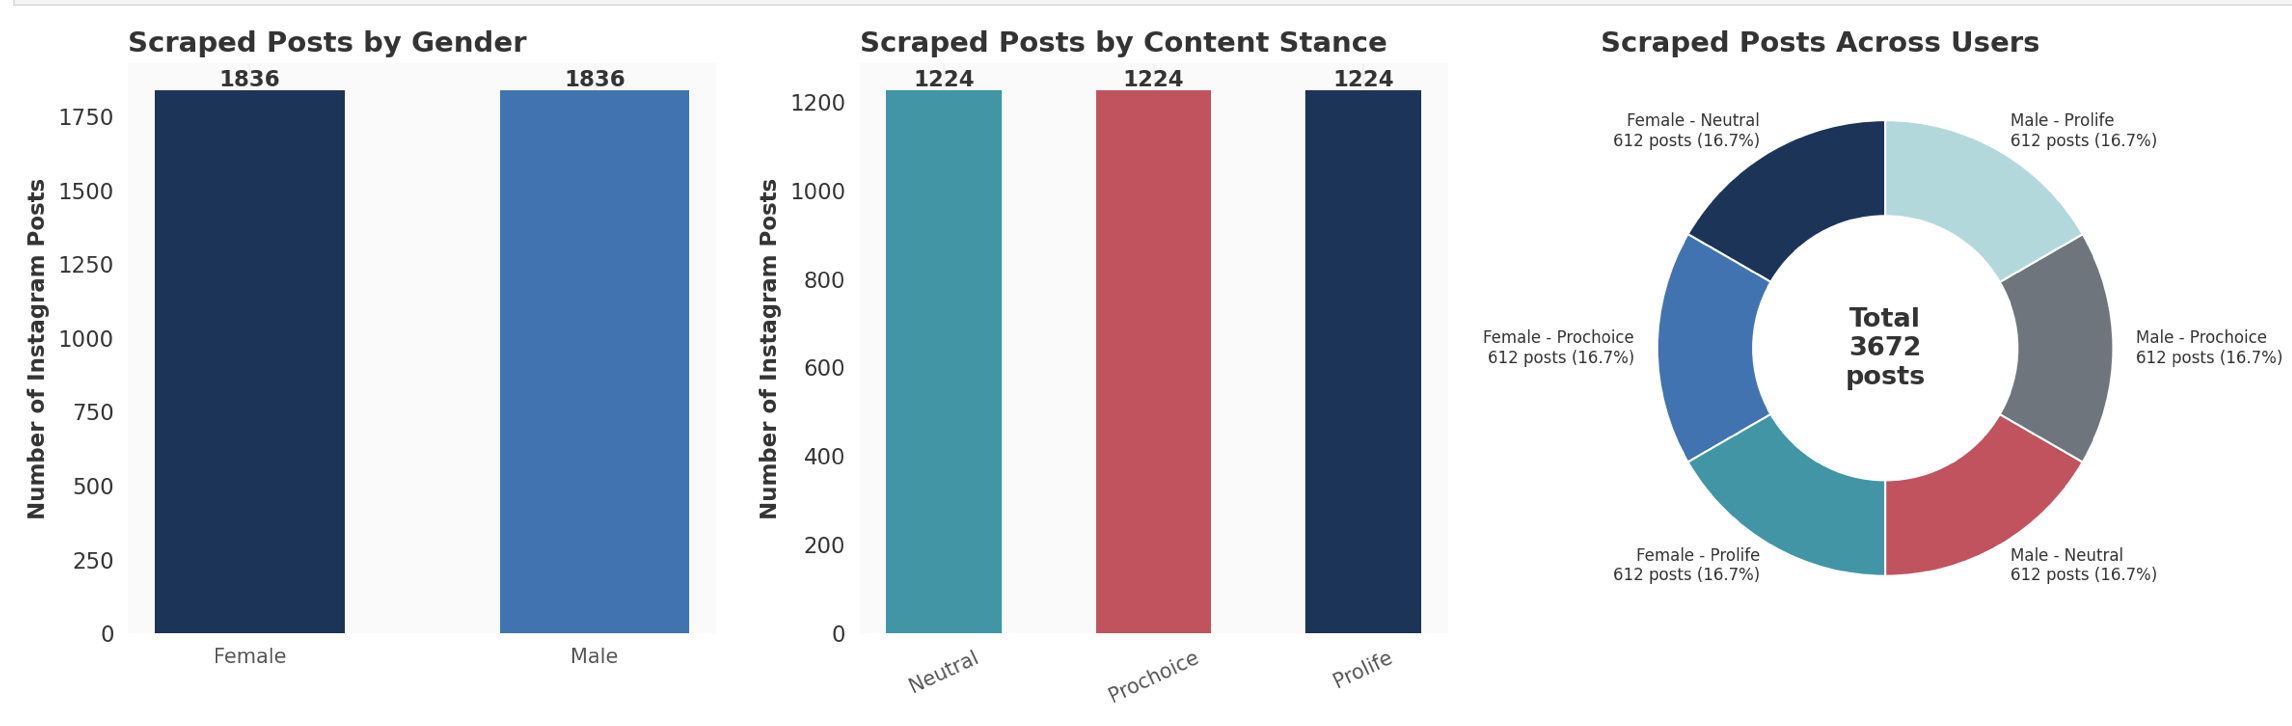
\includegraphics[width=0.9\textwidth]{plots/posts_distribution.png}
\caption{Distribution of posts across gender and stance categories.}
\label{fig:posts_distribution}
\end{figure}


Across all posts, the dataset records 5,721,684 likes and 218,619 comments. Engagement is highly skewed, with posts receiving an average of 9,349 likes and 357 comments, compared to medians of 866 likes and 53 comments, respectively. This difference highlights substantial variation in engagement levels across posts.

\begin{figure}[!htbp]
\centering
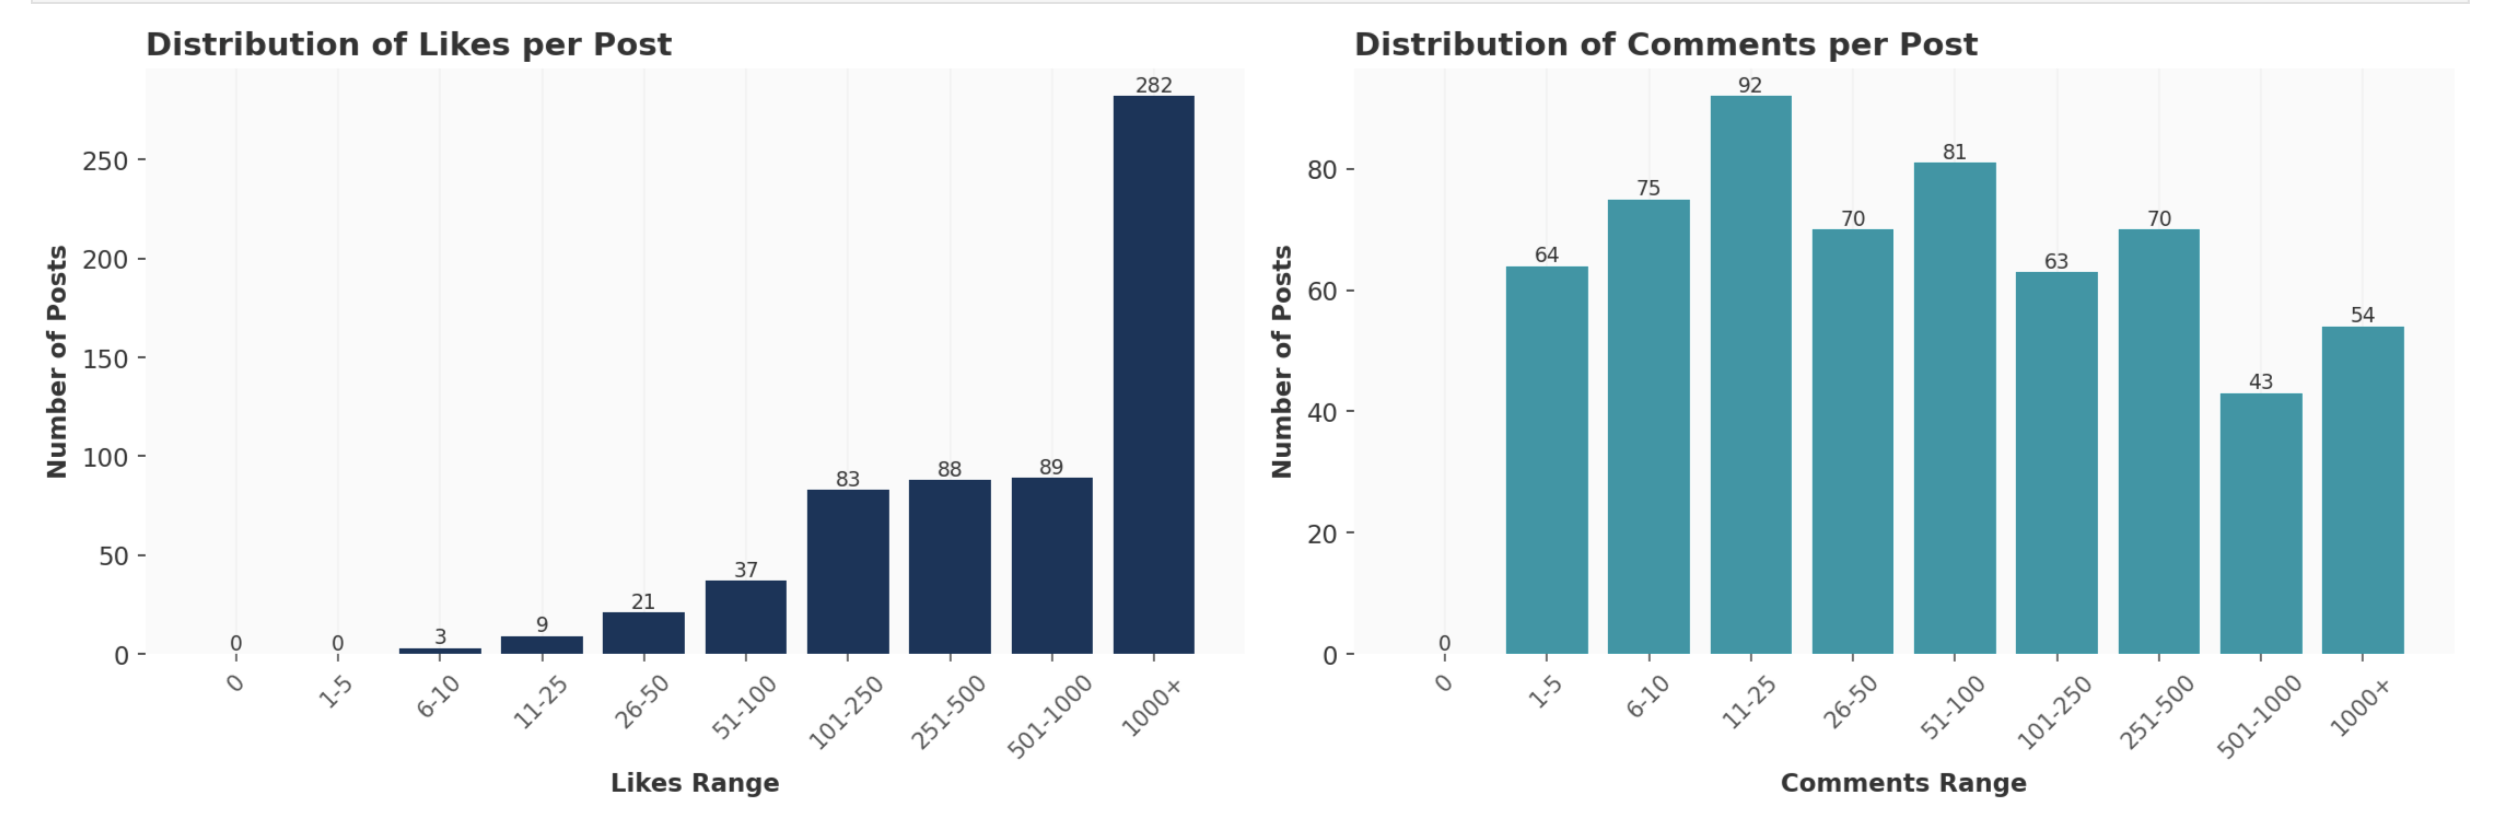
\includegraphics[width=0.9\textwidth]{plots/engagement_distribution.png}
\caption{Distribution of posts according to likes and comments engagement levels.}
\label{fig:engagement_distribution}
\end{figure}

The dataset covers the period from April 2018 to July 2026, encompassing approximately nine years of Instagram activity. This temporal span allows for the examination of variations in posting and interaction patterns over an extended period, while accounting for potential shifts in online discourse and platform dynamics. Figure~\ref{fig:temporal_distribution} presents the temporal distribution of posts included in the dataset.

\begin{figure}[!htbp]
\centering
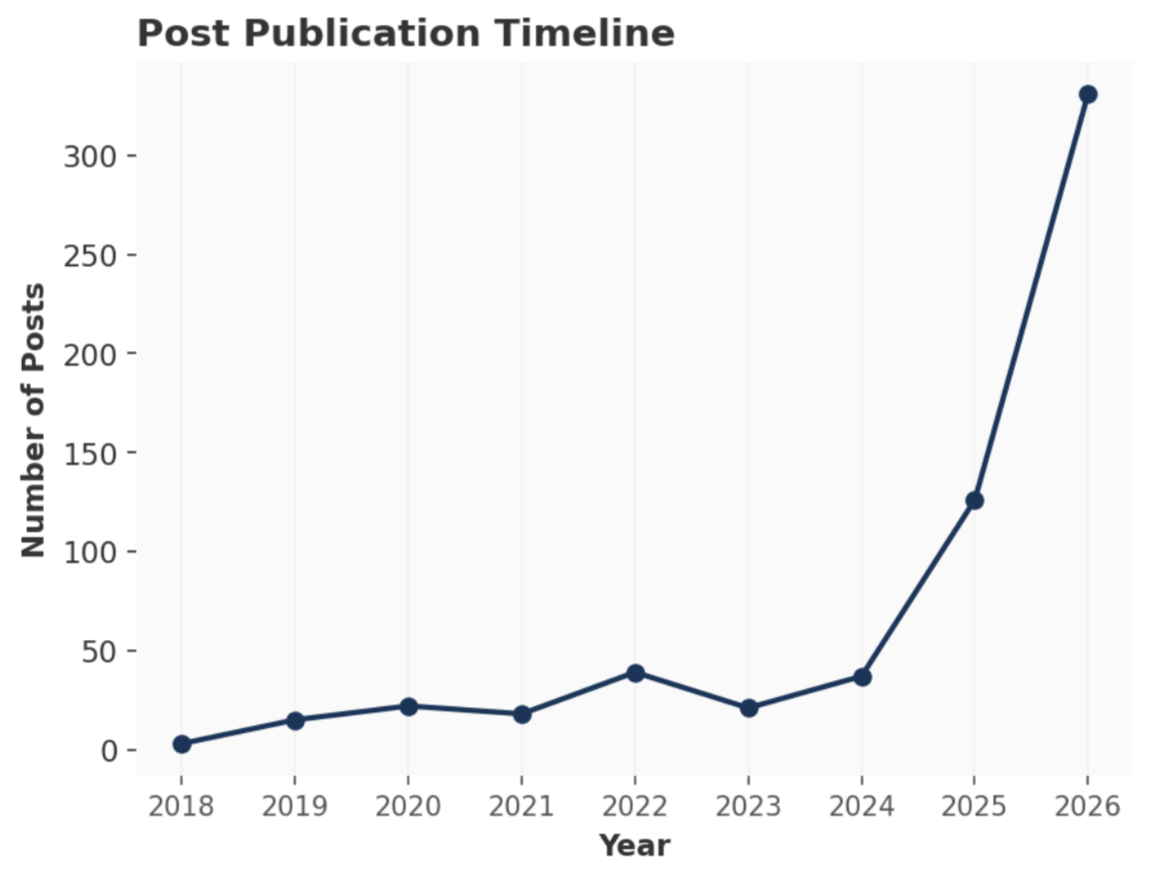
\includegraphics[width=0.85\textwidth]{plots/Post_Publication_timeline.png}
\caption{Temporal distribution of posts in the dataset.}
\label{fig:temporal_distribution}
\end{figure}


Finally, publisher and user verification statuses were analysed to describe the distribution of verified and non-verified accounts within the dataset. At the post level, 414 posts (67.6\%) were published by non-verified accounts, while 198 posts (32.4\%) originated from verified publishers. At the comment level, verified users accounted for only 2.11\% of all interactions, indicating that engagement was predominantly generated by non-verified accounts.


\begin{figure}[!htbp]
\centering
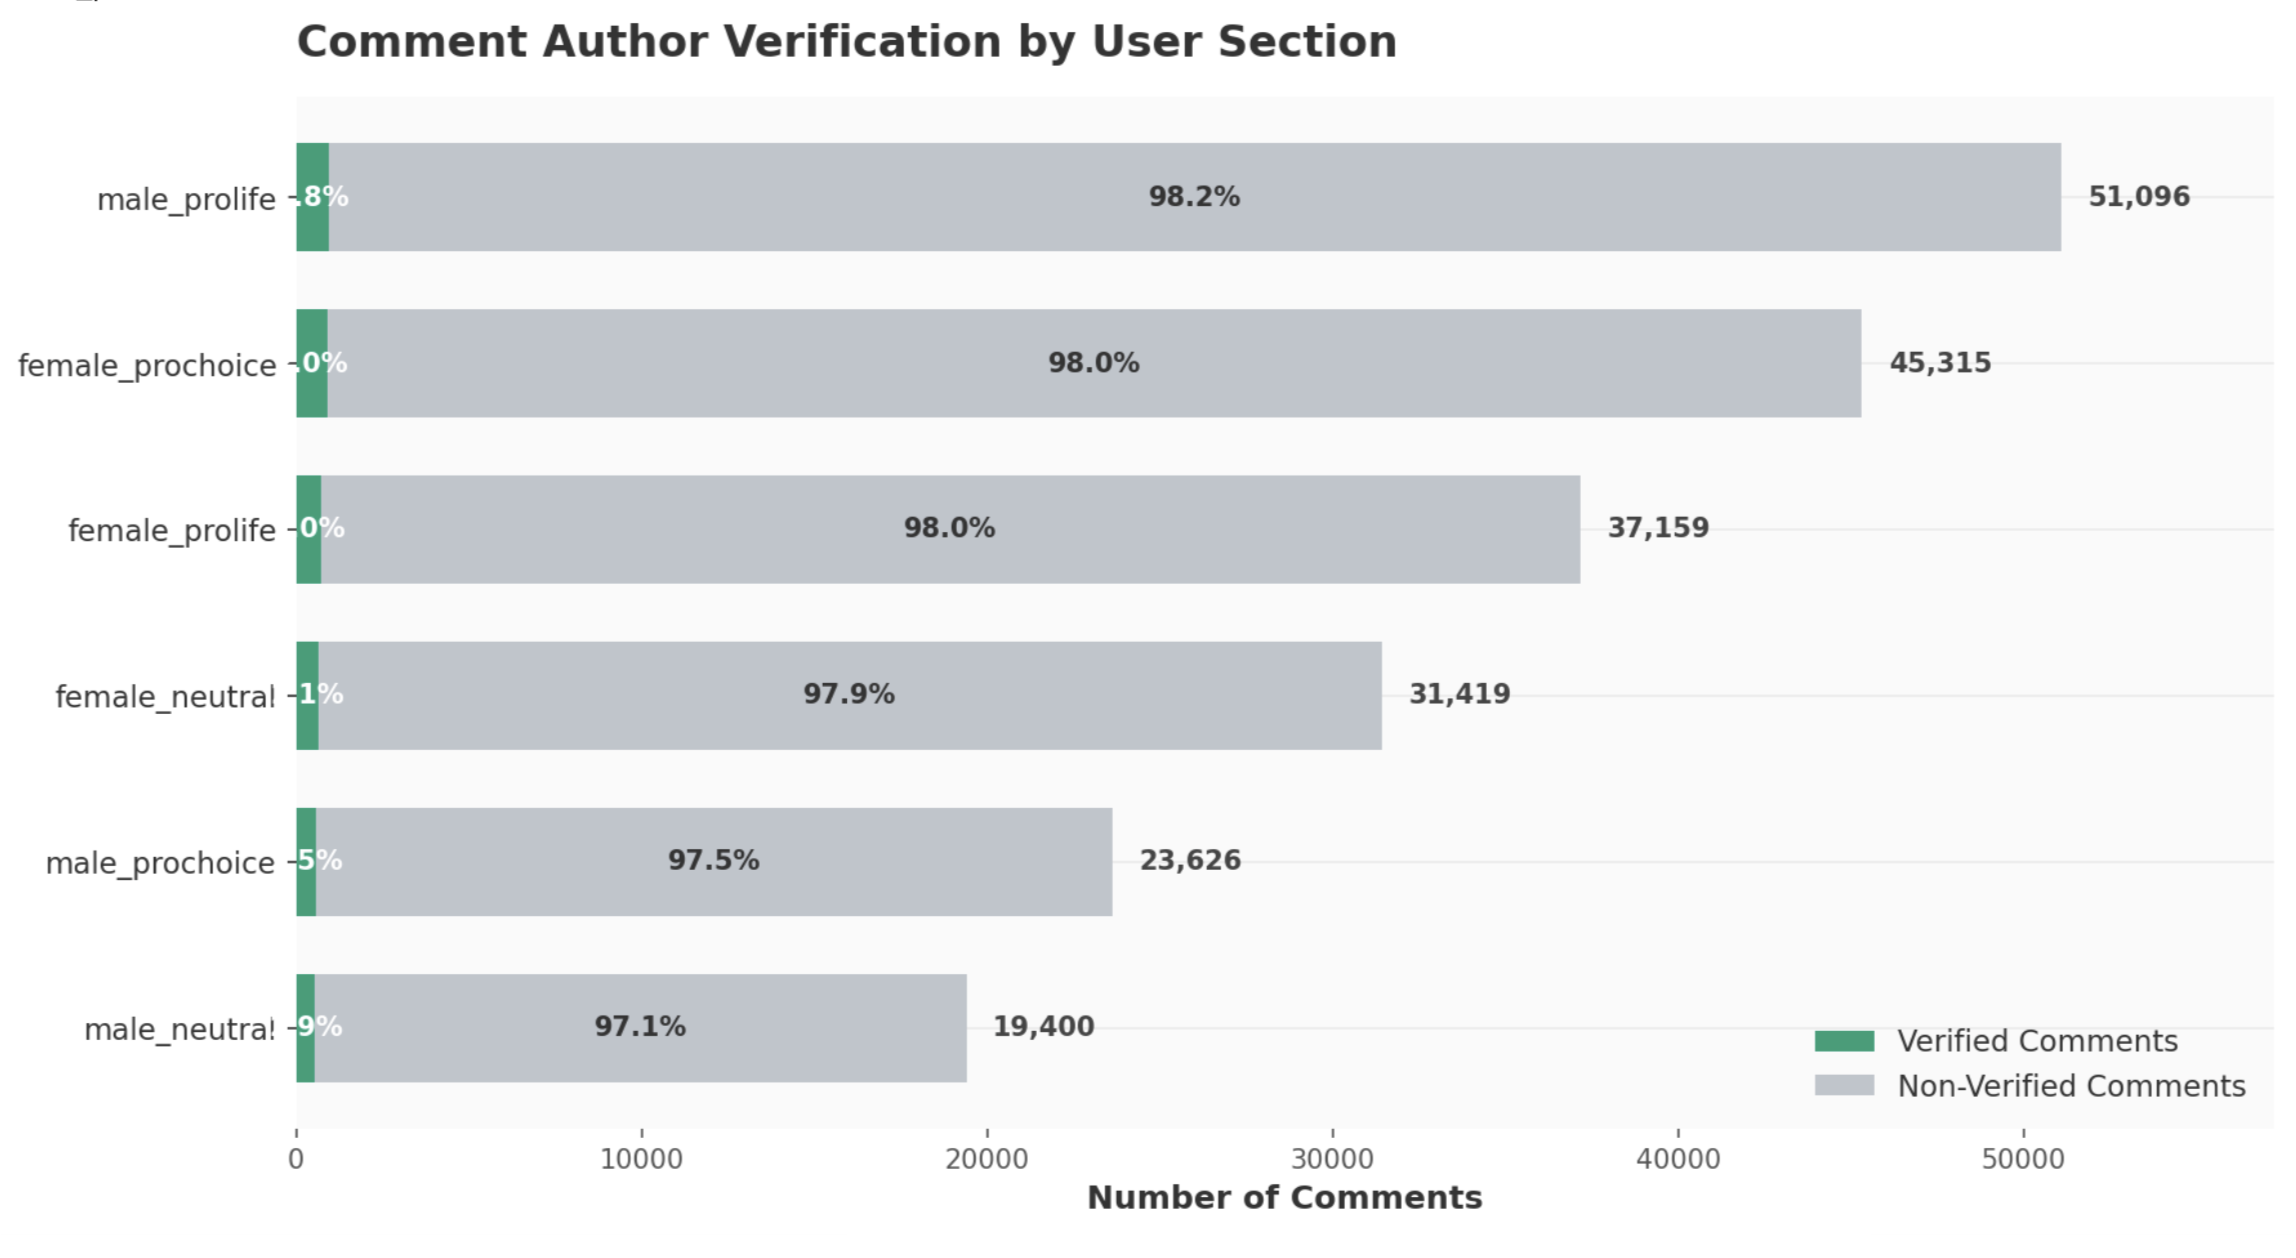
\includegraphics[width=0.9\textwidth]{plots/verification_distribution.png}
\caption{Distribution of verified and non-verified comments across user categories.}
\label{fig:verification_distribution}
\end{figure}

\subsection{Research Objectives}

This study investigates factors influencing divergence in Instagram interactions, specifically examining how engagement metrics, user attributes, and temporal factors relate to divergence scores across different demographic and ideological positions.
